\documentclass[a4paper,11pt,openany]{book}
\usepackage[utf8]{inputenc}
\usepackage[left=2.54cm,top=2.54cm,right=2.54cm,bottom=2.54cm]{geometry}
\usepackage[spanish]{babel}
\usepackage{amsmath}
\usepackage{amsfonts}
\usepackage{amssymb}
\usepackage{graphicx}
\usepackage{color}
\usepackage[usenames,dvipsnames]{xcolor}
\usepackage{pifont}
\usepackage{marvosym}
\newtheorem{teo}{Teorema}
\newtheorem{ejemplo}{Ejemplo}
\newtheorem{defi}{Definición}
\newtheorem{coro}{Corolario}
\newtheorem{prueba}{Prueba}
\newtheorem{exmp}{Example}[section]
\newtheorem{ejer}{Ejercicio}[section]
\def\proof{\paragraph{\textsf{Demostración.} }}
\def\endproof{\hfill $\blacksquare$ \\}
\usepackage{multirow, array} % para las tablas
\usepackage{multirow}
\usepackage{tabularx}
\usepackage{float} % para usar [H]
\usepackage{tikz}
\usepackage[all]{xy}
\usepackage{cancel}
\usetikzlibrary{positioning}
\usepackage{enumitem}
\newcommand*{\itembolasazules}[1]{% bolas 3D
\footnotesize\protect\tikz[baseline=-3pt]%
\protect\node[scale=.7, circle, shade, ball
color=green]{\color{white}\Large\bf#1};}
\usepackage{tcolorbox} 
\tcbuselibrary{listingsutf8}
\newtcolorbox[auto counter,number within=section]{example}[2][]
{colback=green!5!white,colframe=green!75!black,fonttitle=\bfseries, title=Ejercicio~\thetcbcounter: #2,#1}
\usepackage{background}
\backgroundsetup{
placement=center,
angle=0,
scale=1.1,
contents= {{
\includegraphics{HojaCuadriculada.png}}}
}
 
 
\begin{document}
\begin{titlepage}
 
\begin{center}
\vspace*{-1in}
\begin{figure}[htb]
\begin{center}

\includegraphics[width=7cm]{ETITC.png}
\end{center}
\end{figure}
 
 
{\sc \huge Escuela Tecnológica Instituto Técnico Central (ETITC)}\\
\vspace*{0.15in}
Facultad de sistemas\\
\vspace*{0.6in}
\begin{Large}
\textbf{Taller 5 : Integrales Complejas y Teorema de Cauchy - Goursat.} \\
\textbf{Matem{\'a}ticas Especiales}\\
\end{Large}
\vspace*{0.3in}
\begin{large}
{\bf Autores} \\
 
\ 
 
Sergio Alejandro Enrrique Caballero Leon\\ 
Johan Alejandro Sogamoso Camacho \\
David Andrés Valero Vanegas \\
\end{large}
\vspace*{0.3in}
 
\end{center}
 
\begin{center}
{\bf Presentado a:} \\
 
\ 
 
Carlos Romero \\
 
\
 
Bogot{\'a}, Noviembre de 2022.
\end{center}
 
\end{titlepage}

\newpage

\definecolor{ao(english)}{rgb}{0.0, 0.5, 0.0}

\graphicspath{ {images/} }

\begin{center}
\textbf{Integrales Complejas}
\end{center}

Evalue las sigientes integrales a lo largo del controno indicado en cada caso.\\

\textcolor{ao(english)}{(\,1\,)} $\bf{\displaystyle\int\limits_{C}\,(5\,-\,z^{2}\,+\,2\,z)\,dz}$.

\begin{center}
     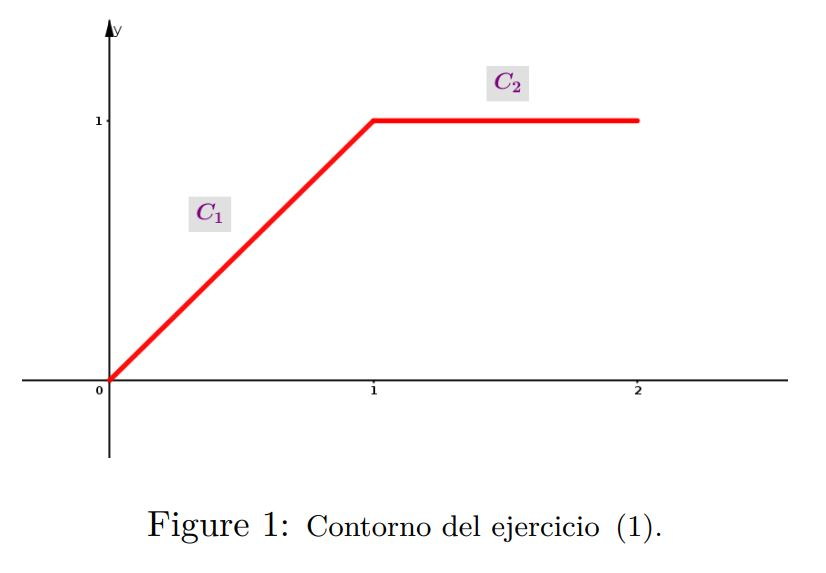
\includegraphics[width=10cm]{figura-1.JPG}
\end{center}

El contorno está dado por:\\

$$C_{1} \quad\iff\quad x\,=\,y,\,0\leq\,x\,\leq\,1,\,y\,=\,0$$

$$C_{2} \quad\iff\quad 1\leq\,x\,\leq\,2,\,y\,=\,1$$

$\bf{\displaystyle\int\limits_{C_{1}}\,f(z)\,dz}$.\\

\textcolor{ao(english)}{\ding{47}\,Paso 1:} Escribir $z$ en terminos del parámetro.

$$z\,=\,x\,+\,i\,y \qquad\iff\qquad z\,=\,x\,+\,i\,x$$

\textcolor{ao(english)}{\ding{47}\,Paso 2:} Escribir $dz$ en terminos del parámetro.

$$\dfrac{dz}{dx}\,=\,1\,+\,i \quad\iff\quad dz\,=\,(1\,+\,i)\,dx$$

\textcolor{ao(english)}{\ding{47}\,Paso 3:} Escribir $f\,(z)$ en terminos del parámetro.

$$f\,(z)\,=\,(5\,-\,z^{2}\,+\,2\,z)\,=\,5\,-\,(x\,+\,i\,x)^{2}\,+\,2\,(x\,+\,i\,x)$$

\textcolor{ao(english)}{\ding{47}\,Paso 4:} Escribir la integral.

$$\bf{\displaystyle\int\limits_{C_{1}}\,f(z)\,dz}\,=\,\displaystyle\int_{0}^{1}\,[5\,-\,(x\,+\,i\,x)^{2}\,+\,2\,(x\,+\,i\,x)]\,(1\,+\,i)\,dx$$

$$=\,(1\,+\,i)\,\displaystyle\int_{0}^{1}\,[5\,-\,(x\,+\,i\,x)^{2}\,+\,2\,(x\,+\,i\,x)]\,dx$$

$$=\,(1\,+\,i)\,\displaystyle\int_{0}^{1}\,[5\,-\,(x^{2}\,+\,2\,x^{2}\,i\,-\,x^{2})\,+\,2\,x\,+\,2\,x\,i)]\,dx$$

$$=\,(1\,+\,i)\,\displaystyle\int_{0}^{1}\,[5\,-\,2\,x^{2}\,i\,+\,2\,x\,+\,2\,x\,i)]\,dx$$

$$=\,(1\,+\,i)\,\left(5\,x\,-\dfrac{2\,x^{3}\,i}{3}\,+\,\dfrac{2\,x^{2}}{2}+\,\dfrac{2\,x^{2}\,i}{2}\bigg|_{0}^{1}\,\right)$$

$$=\,(1\,+\,i)\,\left(5\,x\,-\dfrac{2\,i}{3}\,+\,1\,+\,\dfrac{3\,i}{3}\bigg|_{0}^{1}\,\right)$$

$$=\,(1\,+\,i)\,\left(6\,+\,\dfrac{i}{3}\right)$$

$$=\,6\,+\,\dfrac{i}{3}\,+\,6\,i\,-\,\dfrac{1}{3} \qquad=\qquad\,\dfrac{17}{3}\,+\,\dfrac{19\,i}{3}$$

$\bf{\displaystyle\int\limits_{C_{2}}\,f(z)\,dz}$.\\

\textcolor{ao(english)}{\ding{47}\,Paso 1:} Escribir $z$ en terminos del parámetro.

$$z\,=\,x\,+\,i\,y \qquad\iff\qquad z\,=\,x\,+\,i$$

\textcolor{ao(english)}{\ding{47}\,Paso 2:} Escribir $dz$ en terminos del parámetro.

$$\dfrac{dz}{dx}\,=\,1 \quad\iff\quad dz\,=\,dx$$

\textcolor{ao(english)}{\ding{47}\,Paso 3:} Escribir $f\,(z)$ en terminos del parámetro.

$$f\,(z)\,=\,(5\,-\,z^{2}\,+\,2\,z)\,=\,5\,-\,(x\,+\,i)^{2}\,+\,2\,(x\,+\,i)$$

\textcolor{ao(english)}{\ding{47}\,Paso 4:} Escribir la integral.

$$\bf{\displaystyle\int\limits_{C_{2}}\,f(z)\,dz}\,=\,\displaystyle\int_{1}^{2}\,[5\,-\,(x\,+\,i)^{2}\,+\,2\,(x\,+\,i)]\,dx$$

$$=\,\displaystyle\int_{1}^{2}\,[5\,-\,(x^{2}\,+\,2\,x\,i\,-\,1)\,+\,2\,x\,+\,2\,i)]\,dx$$

$$=\,\displaystyle\int_{1}^{2}\,[5\,-\,x^{2}\,-\,2\,x\,i\,+\,1\,+\,2\,x\,+\,2\,i)]\,dx$$

$$=\,\left(6\,x\,-\dfrac{x^{3}}{3}\,-\,\dfrac{2\,x^{2}\,i}{2}+\,\dfrac{2\,x^{2}}{2}\,+\,2\,x\,i\,\right)\bigg|_{1}^{2}$$

$$=\,\left(12\,-\dfrac{8}{3}\,-\,4\,i\,+\,4\,+\,4\,i\,\right)\,-\,\left(6\,-\dfrac{1}{3}\,-\,i\,+\,1\,+\,2\,i\right)$$

$$=\,12\,-\dfrac{8}{3}\,-\,4\,i\,+\,4\,+\,4\,i\,-\,6\,+\dfrac{1}{3}\,+\,i\,-\,1\,-\,2\,i$$

$$=\,9\,-\,\dfrac{8}{3}\,-\,3\,i\,+\,\dfrac{1}{3} \qquad=\qquad\,\dfrac{20}{3}\,-\,i$$

$$\bf{\displaystyle\int\limits_{C}\,=\,\displaystyle\int\limits_{C_{1}}\,+\,\displaystyle\int\limits_{C_{2}}\,=\,\dfrac{17}{3}\,+\,\dfrac{19\,i}{3}\,+\,\dfrac{20}{3}\,-\,i\,=\,\dfrac{37}{3}\,+\,\dfrac{16\,i}{3}}$$

\textcolor{ao(english)}{(\,2\,)} $\bf{\displaystyle\int\limits_{C}\,(2\,\overline{z}\,-\,z)\,dz}$, \qquad donde \qquad $C$ es $x\,=\,-\,t \quad;\quad y\,=\,t^{2}\,+\,2 \quad;\quad 0\,\leq\,t\,\leq\,2$.\\

\textcolor{ao(english)}{\ding{47}\,Paso 1:} Escribir $z$ en terminos del parámetro.

$$z\,(t)\,=\,-\,t\,+\,i\,(t^{2}\,+\,2) \iff z\,(t)\,=\,-\,t\,+\,i\,t^{2}\,+\,2\,i)$$

\textcolor{ao(english)}{\ding{47}\,Paso 2:} Escribir $dz$ en terminos del parámetro.

$$\dfrac{dz}{dt}\,=-\,1\,+\,2\,i\,t \quad\iff\quad dz\,=\,(-\,1\,+\,2\,i\,t)\,dt$$

\textcolor{ao(english)}{\ding{47}\,Paso 3:} Escribir $f\,(z)$ en terminos del parámetro.

$$f\,(z)\,=\,2\,\overline{z}\,-\,z\,=\,2(-\,t\,-\,i(t^{2}\,+\,2))\,-\,(\,-\,t\,+\,i(t^{2}\,+\,2))\, $$

$$f\,(z)\,= \,-\,2\,t\,-\,2\,i\,t^{2}\,-\,4\,i\,+\,t\,-\,i\,t^{2}\,-2\,i  $$

$$f\,(z)\,= \,-\,3i\,t^{2}\,-\,t\,-\,6i\,  $$

\textcolor{ao(english)}{\ding{47}\,Paso 4:} Escribir la integral.

$$\displaystyle\int\limits_{C}\,2\,\overline{z}\,-\,z\,dz\,=\,\displaystyle\int_{0}^{2}\,(-\,3i\,t^{2}\,-\,t\,-\,6i\,)\,(-\,1\,+\,2\,i\,t)\,dt\,$$

$$\displaystyle\int_{0}^{2}\,3\,i\,t^{2}\,+\,6\,t^{3}\,+\,t\,-\,2\,i\,t^{2}\,+\,6\,i\,+\,12\,t\, dt\,$$

$$=\,\left(  3i\dfrac{t^{3}}{3}\,+\,6\dfrac{t^{4}}{4}\,+\,\dfrac{t^{2}}{2}\,-\,2i\dfrac{t^{3}}{3}\,+\,6it\,+\,12t\right)\bigg|_{0}^{2}\,=\,8i\,+\,24\,+\,2\,-\,\dfrac{16i}{3}\,+\,12i\,+\,24$$

$$=\,50\,+\,20i\,-\,\dfrac{16i}{3}\,\,=\boxed{50\,+\,\dfrac{44i}{3}} $$

\textcolor{ao(english)}{(\,3\,)} $\bf{\displaystyle\int\limits_{C}\,z^{2}\,dz}$, \qquad donde \qquad $C$ es $z\,(t)\,=\,3\,t\,-\,2\,i\,t \quad;\quad -\,2\,\leq\,t\,\leq\,2$.\\

\textcolor{ao(english)}{\ding{47}\,Paso 1:} Escribir $z$ en terminos del parámetro.

$$z\,(t)\,=\,3\,t\,-\,2\,i\,t$$

\textcolor{ao(english)}{\ding{47}\,Paso 2:} Escribir $dz$ en terminos del parámetro.

$$\dfrac{dz}{dt}\,=\,3\,-\,2\,i \quad\iff\quad dz\,=\,(3\,-\,2\,i)\,dt$$

\textcolor{ao(english)}{\ding{47}\,Paso 3:} Escribir $f\,(z)$ en terminos del parámetro.

$$f\,(z)\,=\,z^{2}\,=\,(3\,t\,-\,2\,i\,t)^{2}\,=\,9\,t^{2}\,-\,12\,i\,t^{2}\,-\,4\,t^{2}\,=\,5\,t^{2}\,-\,12\,i\,t^{2}$$

\textcolor{ao(english)}{\ding{47}\,Paso 4:} Escribir la integral.

$$\displaystyle\int\limits_{C}\,z^{2}\,dz\,=\,\displaystyle\int_{-\,2}^{2}\,(5\,t^{2}\,-\,12\,i\,t^{2})\,(3\,-\,2\,i)\,dt\,=\,(3\,-\,2\,i)\,\displaystyle\int_{-\,2}^{2}\,(5\,t^{2}\,-\,12\,i\,t^{2})\,dt$$

$$=\,(3\,-\,2\,i)\,\left(\dfrac{5\,t^{3}}{3}\,-\,4\,i\,t^{3}\right)\bigg|_{-\,2}^{2}\,=\,(3\,-\,2\,i)\,\left[\dfrac{5(2^{3})}{3}\,-\,\dfrac{5((-\,2)^{3})}{3}\,-\,(4\,i\,(2^{3})\,-\,4\,i\,((-\,2)^{3}))\right]$$

$$=\,(3\,-\,2\,i)\,\left[\dfrac{40}{3}\,+\,\dfrac{40}{3}\,-\,(32\,i\,+\,32\,i)\right]\,=\,(3\,-\,2\,i)\,\left(\dfrac{80}{3}-\,64\,i\right)$$

$$=\,80\,-\,192\,i\,-\,\dfrac{160\,i}{3}\,-\,128\,=\,\boxed{-\,48\,-\,\dfrac{736\,i}{3}}$$

\textcolor{ao(english)}{(\,4\,)} $\bf{\displaystyle\oint\limits_{C}\,(2\,z\,-\,1)\,dz}$.

\begin{center}
     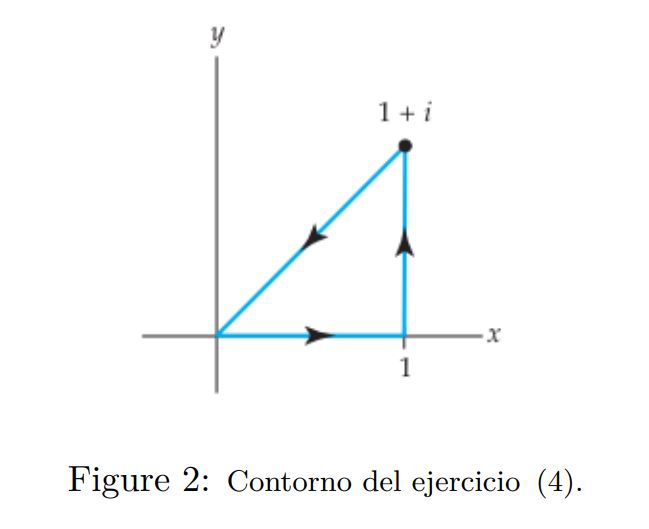
\includegraphics[width=8cm]{figura-2.JPG}
\end{center}

$$\displaystyle\oint\limits_{C_{1}}\,(2\,z\,-\,1)\,dz \quad;\quad \,0\,\leq\,x\,\leq\,1 \quad;\quad y\,=\,0 $$

$$ z\,=\,x\,+\,iy\,\iff \,z\,=\,x\, $$

$$ \dfrac{dz}{dx}\,=\,1\, \iff dz\,=\,dx $$

$$ \,f(x)\,=\,2(x)-1 = \displaystyle\int_{0}^{1}\,2\,x\,-\,1\,dx\,=\,\dfrac{2\,x^{2}}{2}\,-\,x \bigg|_{0}^{1}\,=\,1\,-\,1\,=\,0$$

$$\displaystyle\oint\limits_{C_{2}}\,(2\,z\,-\,1)\,dz \quad;\quad \,0\,\leq\,y\,\leq\,1 \quad;\quad x\,=\,1$$

$$ z\,=\,x\,+\,iy\,\iff \,z\,=\,1\,+\,i\,y$$

$$ \dfrac{dz}{dy}\,=0\,+\,i\, \iff dz\,=\,i\,dy$$

$$ \,f(x)\,=\,2(\,1\,+\,i\,y\,)-1 = 1\,+\,2\,i\,y = \displaystyle\int_{0}^{1}\,(1\,+\,2\,i\,y)\,i\,dy$$

$$ \displaystyle\int_{0}^{1}\,i\,-\,2y\,dy\,=iy\,-\,\dfrac{2\,y^{2}}{2}\, \bigg|_{0}^{1}\,=\,i\,-\,1\,=\,-\,1\,+\,i$$
---

$$\displaystyle\oint\limits_{C_{3}}\,(2\,z\,-\,1)\,dz \quad;\quad \,1\,\leq\,y\,\leq\,0 \quad;\quad x\,=\,y $$

$$ z\,=\,x\,+\,iy\,\iff \,z\,=\,y\,+\,i\,y $$

$$ \dfrac{dz}{dy}\,= 1\,+\,i\, \iff dz\,=1\,+\,i\,\,dy $$

$$ \,f(x)\,=\,2(y\,+\,i\,y\,)-1 = \displaystyle\int_{1}^{0}\,2(y+iy)-1\,dz$$

$$ =\displaystyle\int_{1}^{0}\,(2y+2iy-1)(1+i)\,\,dy\,= \displaystyle\int_{1}^{0}\,4\,i\,y\,-\,1\,-\,i\,\,dy\,= \dfrac{\,4\,i\,y^{2}}{2}\,-\,y\,-\,i\,y\, \bigg|_{1}^{0}$$

$$ = -\,(\,2\,i\,-\,1\,-\,i\,)\,=\,-\,1\,+\,i $$

$$\displaystyle\oint\limits_{C} = \displaystyle\oint\limits_{C_{1}} + \displaystyle\oint\limits_{C_{2}} +\displaystyle\oint\limits_{C_{3}} = \,0\,-\,1\,+\,i\,-\,1+i\, = \boxed{\,-\,2\,+\,2\,i\,} $$


\begin{center}
\textbf{Teoremas de Cauchy y de Cauchy - Goursat}
\end{center}

Ejercicios \textbf{(\,5\,)} al \textbf{(\,7\,)}. Usando los procedimientos vistos en clase, \textbf{muestre y justifique} por qué $\oint_{C}\,f\,(z)\,dz\,=\,0$, donde $f$ es la función dada y $C$ es el círculo $|\,z\,|\,=\,1$, Además, dibuje el círculo en el plano complejo e indique (si lo hay), él o los puntos donde $f$ es indeterminada.\\

\textcolor{ao(english)}{(\,5\,)} $\bf{f\,(z)\,=\,z^{3}\,-\,1\,+\,3\,i}$.

\textcolor{ao(english)}{(\,6\,)} $\bf{f\,(z)\,=\,\dfrac{z}{2\,z\,+\,3}}$.

\textcolor{ao(english)}{\ding{46}} Grafica.

\begin{center}
     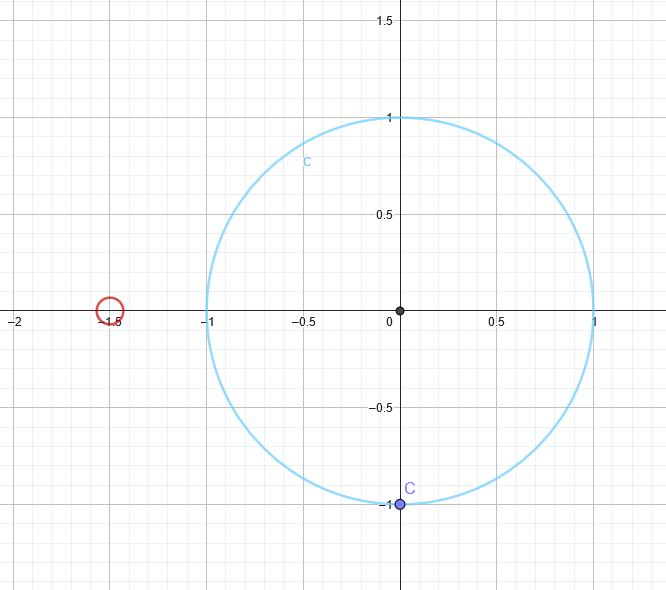
\includegraphics[width=8cm]{Gra-Ej-6.png}
\end{center}

\textcolor{ao(english)}{\ding{46}} Justificación.\\

Dado que el punto $z=-\dfrac{3}{2}$ donde la funcion es indeterminada esta fuera del contorno $C$
y la funcion  $f\,(z)\,=\,\dfrac{z}{2\,z\,+\,3}$ es analitica, por ende:

$$\oint\limits_{C}\,f\,(z)\,dz\,=\,0$$

\textcolor{ao(english)}{(\,7\,)} $\bf{f\,(z)\,=\,\dfrac{e^{z}\,+\,2\,i}{(z^{2}\,-\,25)\,(z^{2}\,+\,9)}}$.\\

\textcolor{ao(english)}{\ding{46}} Grafica.

\begin{center}
     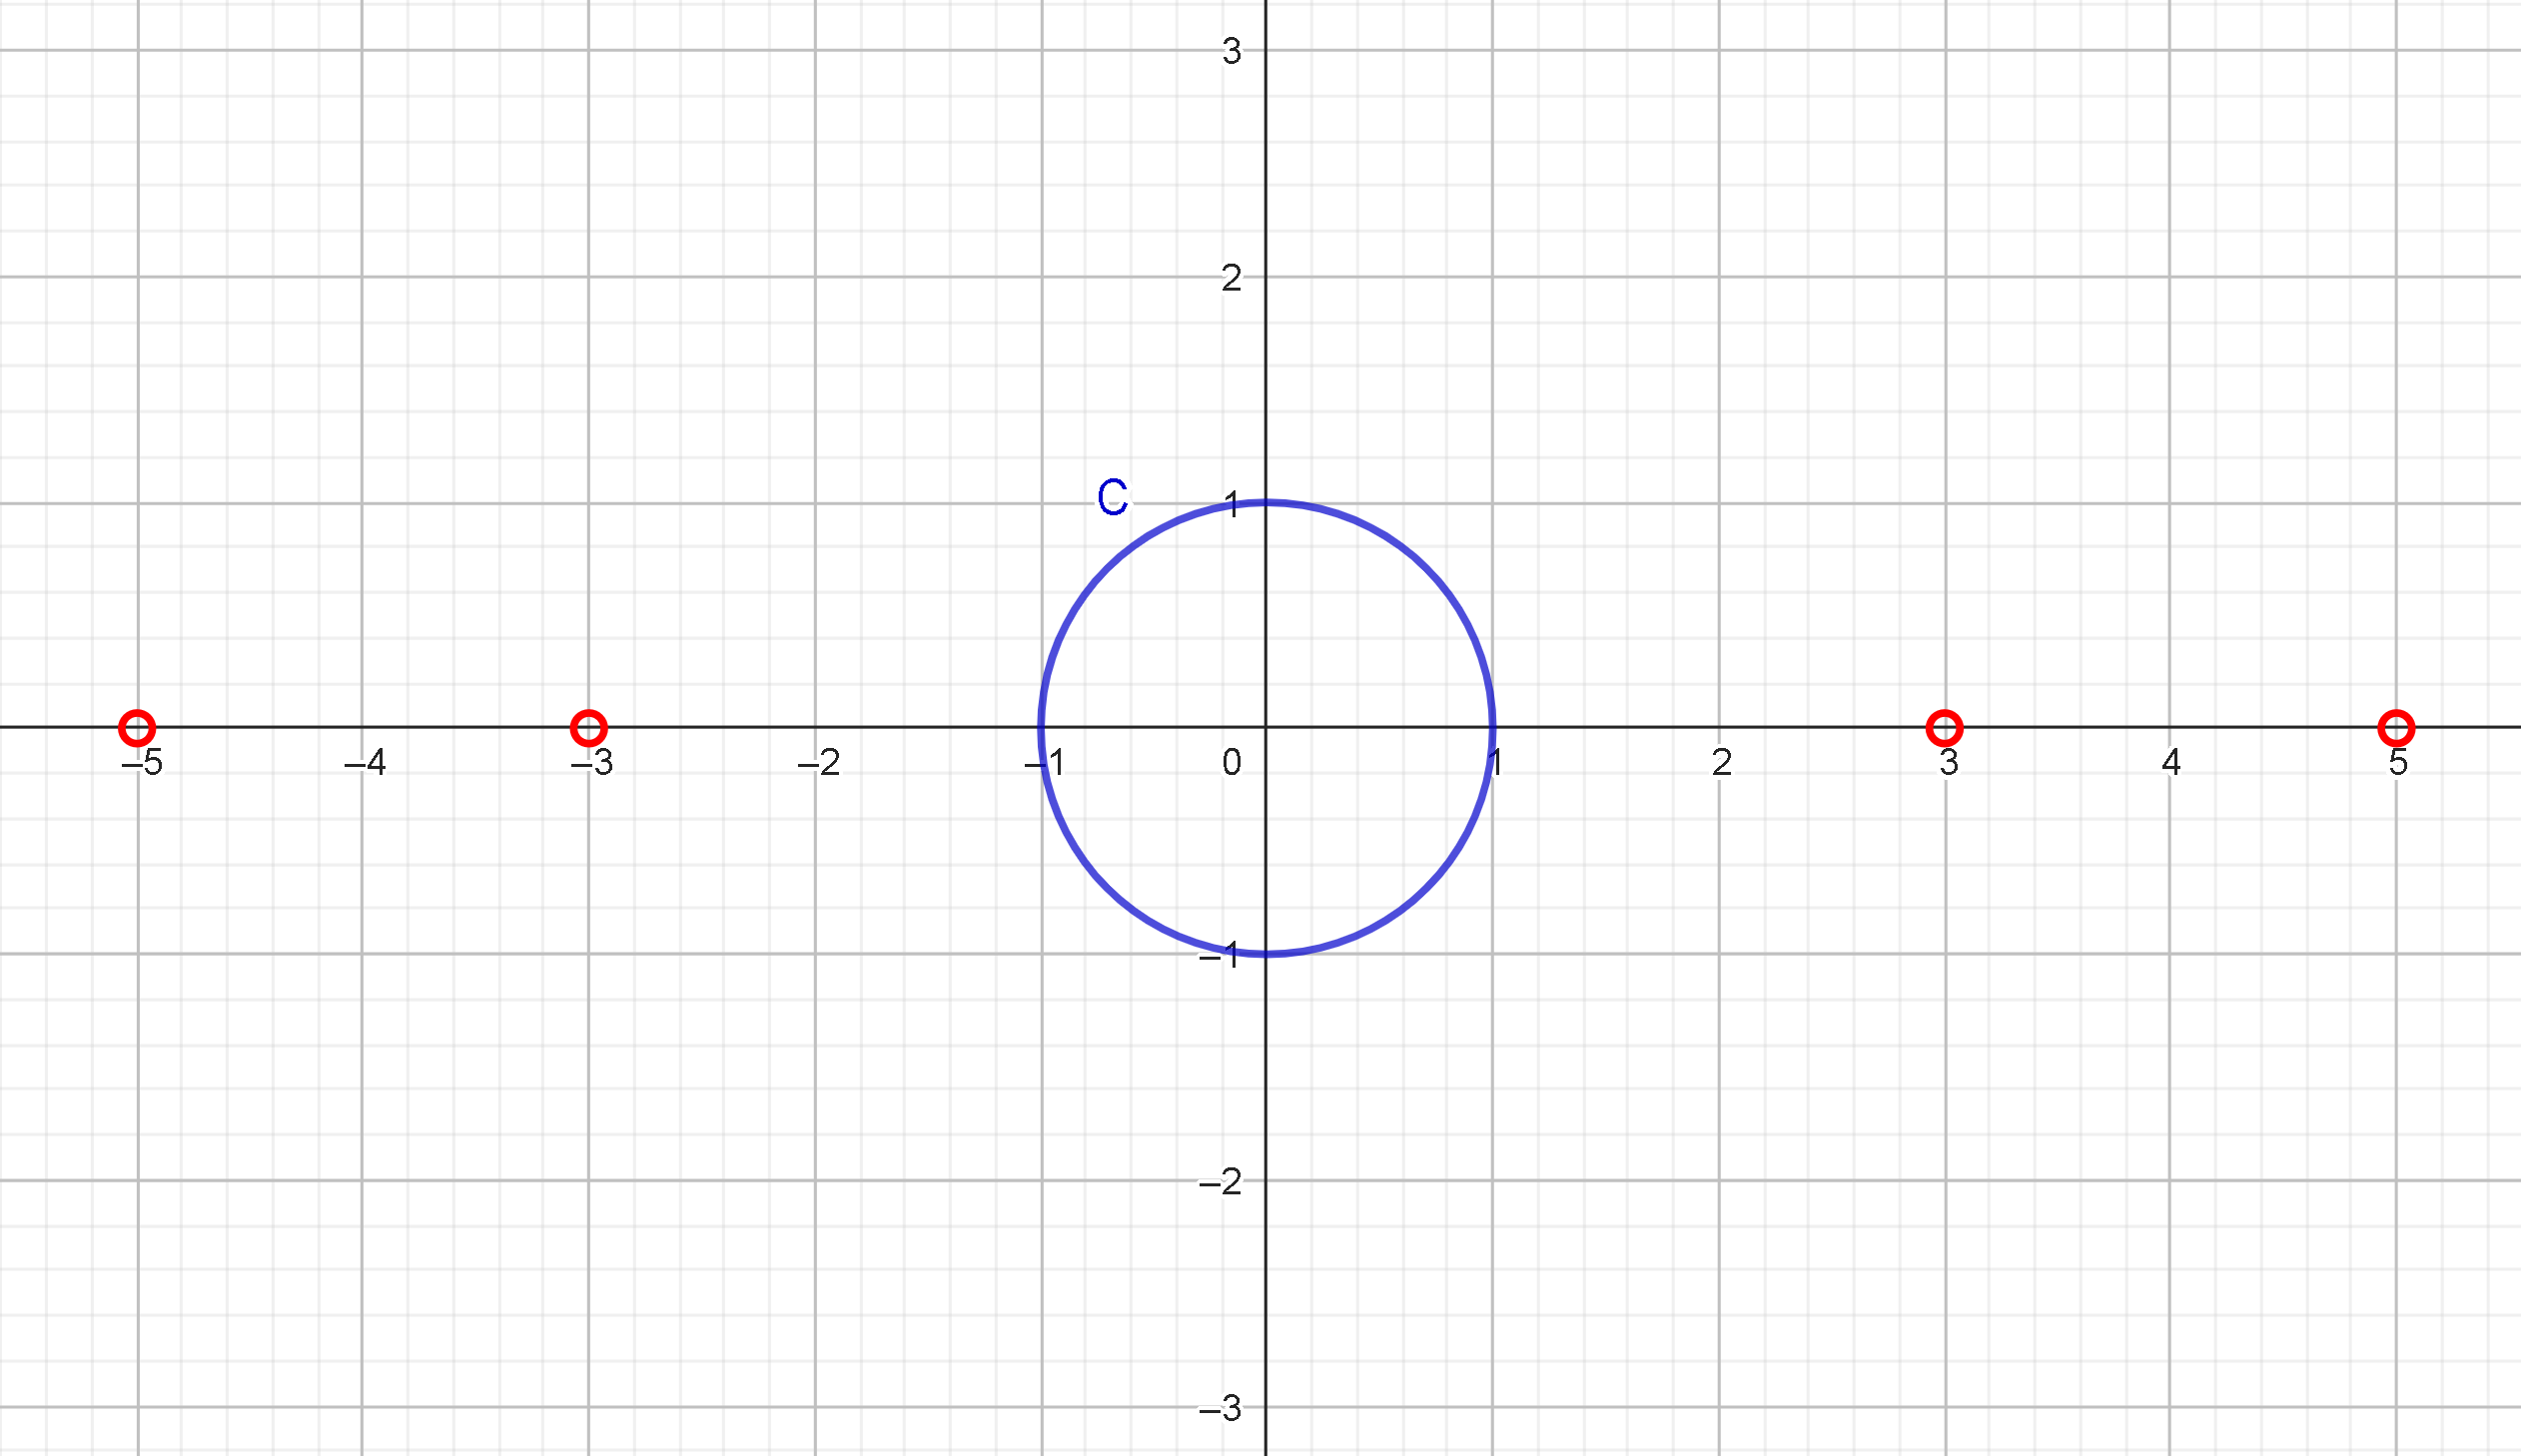
\includegraphics[width=15cm]{Gra-Ej-7.png}
\end{center}

\textcolor{ao(english)}{\ding{46}} Justificación.\\

Es analitica la función $f\,(z)$ en todo $z\,\in\,\mathnormal{Dom\,(f)}$ exceptuando los puntos donde está es indeterminada que son: $z\,=\,-\,5$, $z\,=\,5$, $z\,=\,-\,3$ y $z\,=\,3$; sin embrago los puntos de indeterminación estan fuera del controno $C$. Por ende:

$$\oint\limits_{C}\,f\,(z)\,dz\,=\,0$$

Ejercicios \textbf{(\,8\,)} al \textbf{(\,10\,)}. Evalúe cada integral dada a continuación usando los procedimientos vistos en clase \textbf{justificando su respuesta}. El controno se muestra en la figura o se indica en el correspondiete ejercicio.\\

\textcolor{ao(english)}{(\,8\,)} $\bf{\displaystyle\oint\limits_{C}\,\dfrac{1}{z}\,dz}$.

\begin{center}
     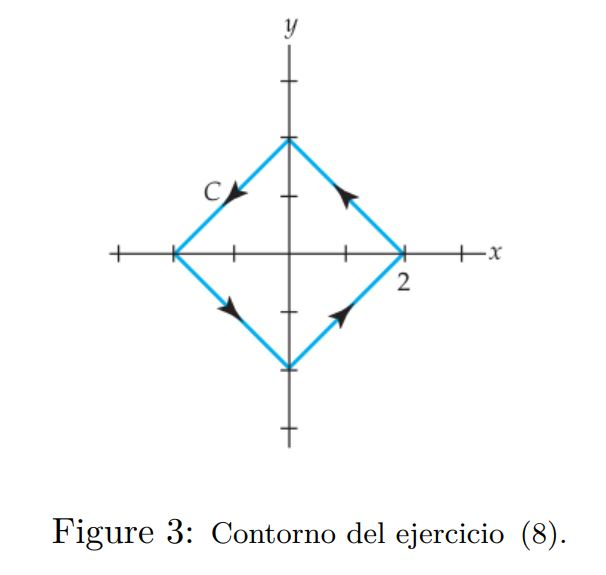
\includegraphics[width=8cm]{figura-3.JPG}
\end{center}

\begin{center}
     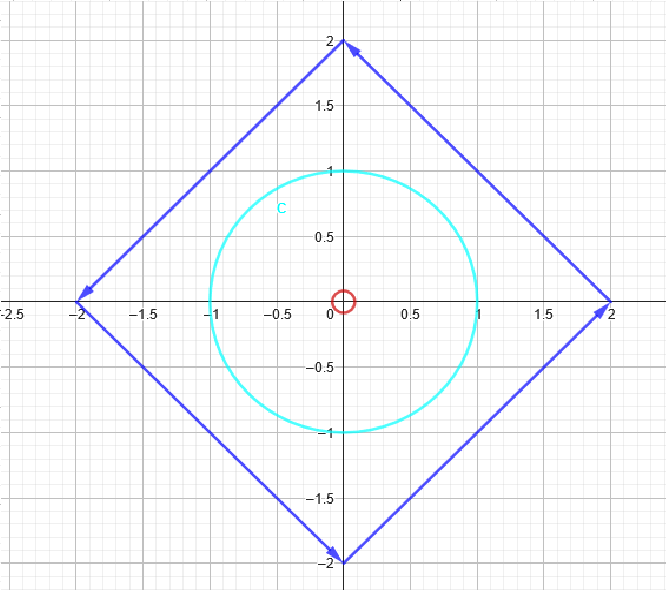
\includegraphics[width=8cm]{Gra-Ej-8.png}
\end{center}

\textcolor{ao(english)}{\ding{46}} Justificación.\\

$\mathnormal{Dom\,(f)}\,=\,\mathbb C\,-\,\{0\}$ es un Dominio doblemente conexo; y ya que $z\,=\,0$ está dentron del controno $C$ el valor de esta integral es:

$$\displaystyle\oint\limits_{C}\,\dfrac{1}{z}\,dz\,=\,2\,\pi\,i$$

\textcolor{ao(english)}{(\,9\,)} $\bf{\displaystyle\oint\limits_{C}\,(z\,+\,\dfrac{1}{z})\,dz}, \qquad |\,z\,|\,=\,2$.

$$\displaystyle\oint\limits_{C}\,(z\,+\,\dfrac{1}{z})\,dz\,=\,\displaystyle\oint\limits_{C}\,\dfrac{z^{2}\,+\,1}{z}\,dz$$

\begin{center}
     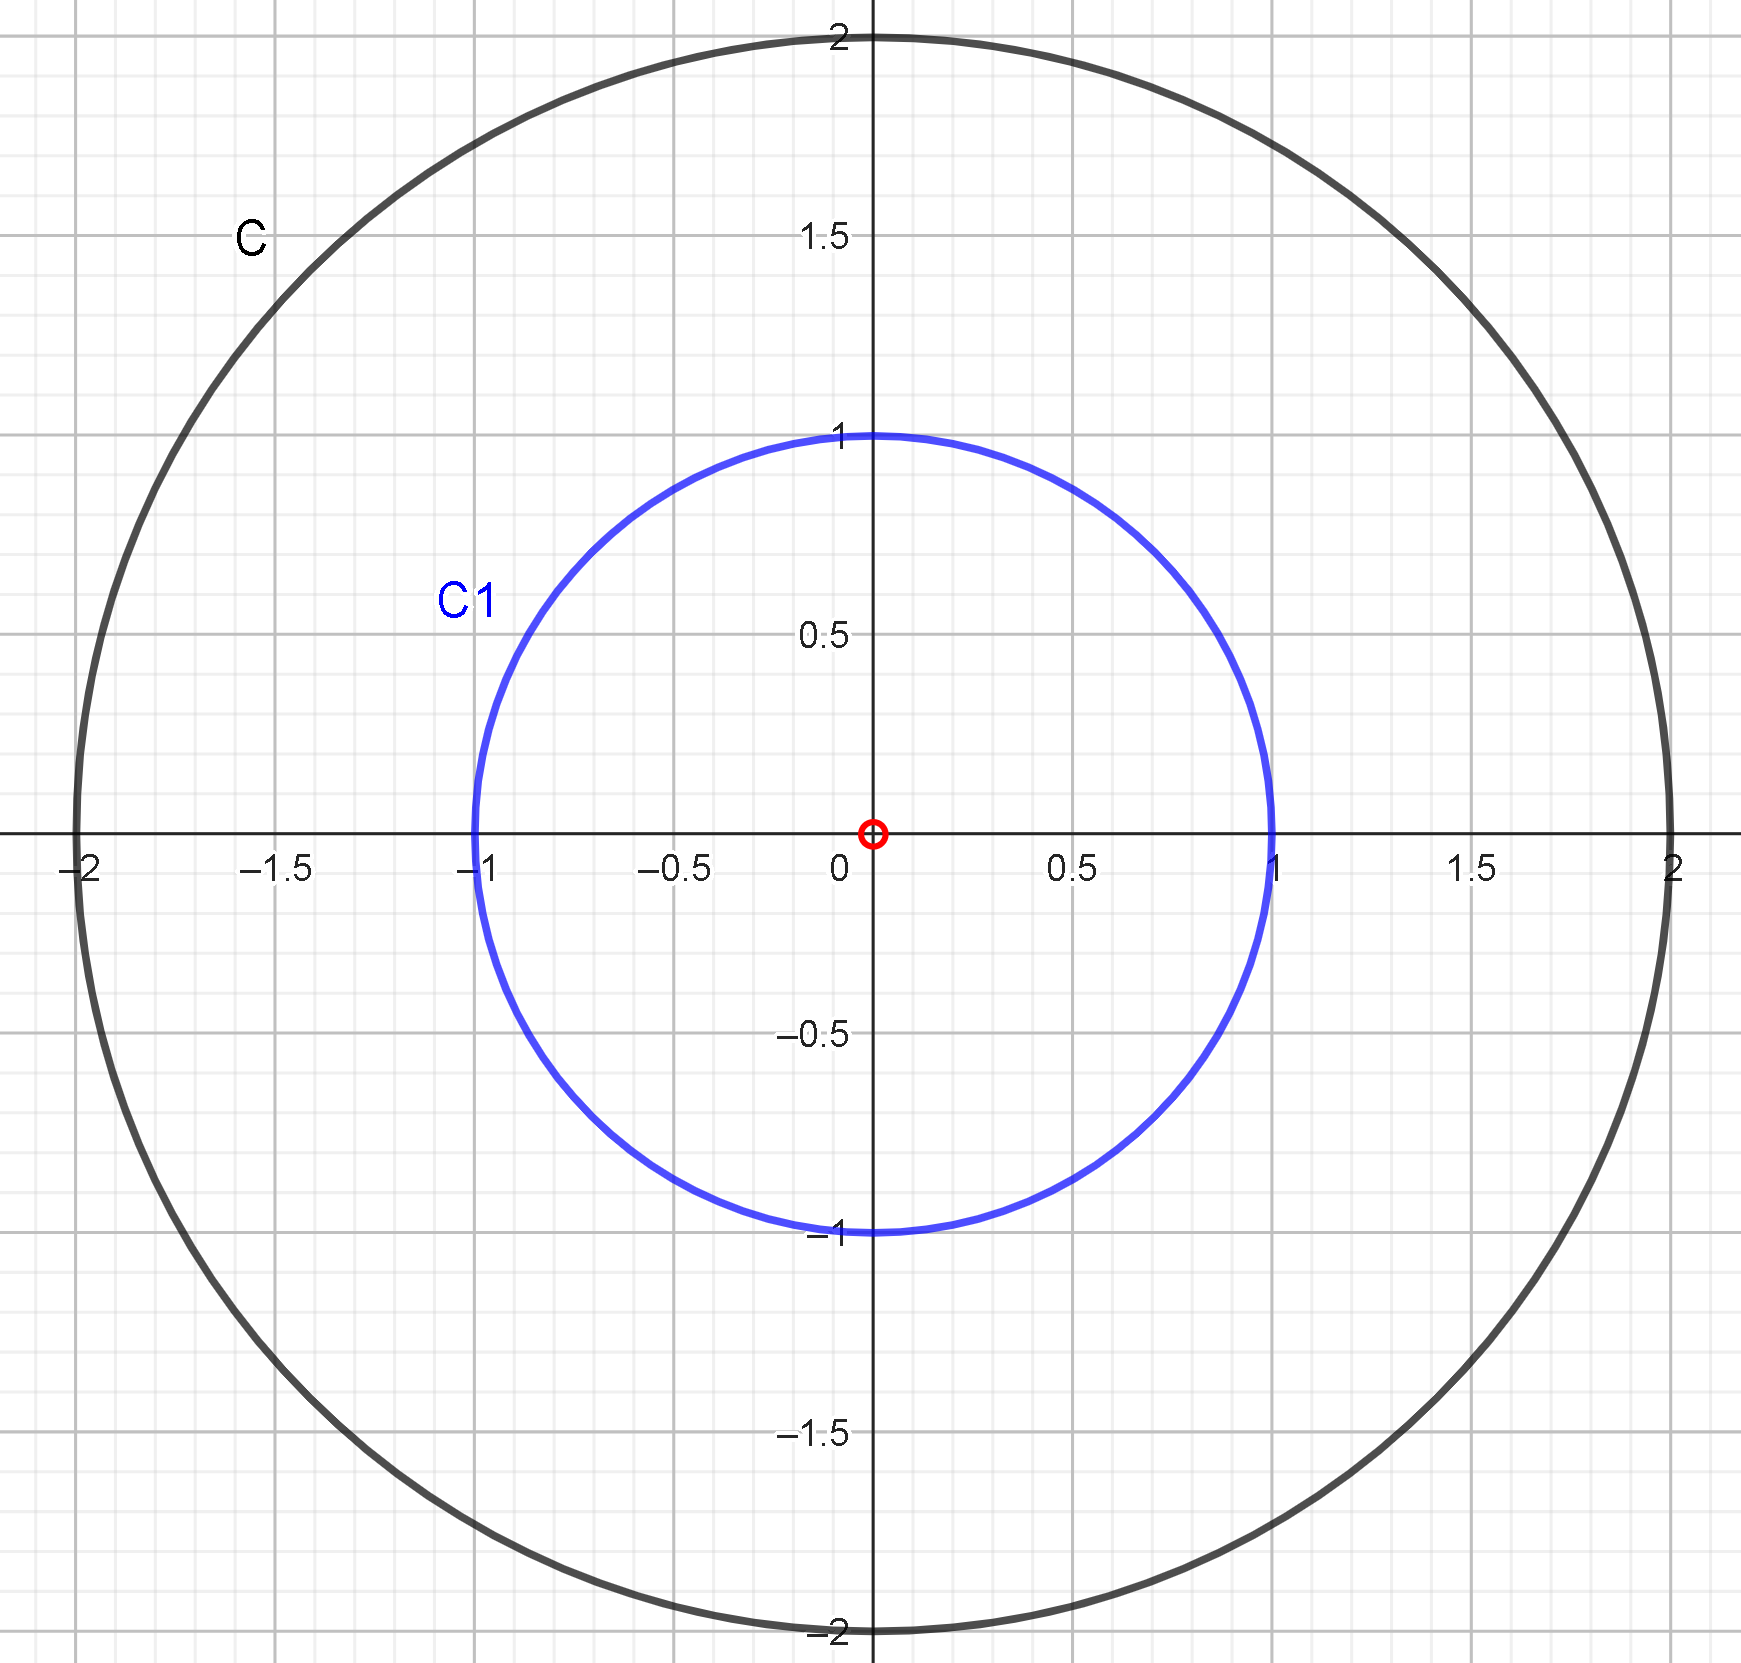
\includegraphics[width=8cm]{Gra-Ej-9.png}
\end{center}

\textcolor{ao(english)}{\ding{46}} Justificación.\\

la función $f\,(z)\,=\,\dfrac{z^{2}\,+\,1}{z}$ tiene $\mathnormal{Dom\,(f)}\,=\,\mathbb C\,-\,\{0\}$.  Vamos a construir un controno $C_{1}$ con centro en $z\,=\,0$, es un circulo de radio 1 con orientación positiva.\\

la ecuación del circulo $C_{1}$ es :

$$|z|\,=\,1$$

Vamos a parametrizar el circulo $C_{1}$:

$$z\,=\,e^{i\,t} \qquad\wedge\qquad 0\,\leq\,t\,\leq\,2\,\pi$$

Escribir $dz$ en treminos del parametro:

$$\dfrac{dz}{dt}\,=\,i\,e^{i\,t} \quad\iff\quad dz\,=\,i\,e^{i\,t}\,dt$$

Usando el principio de deformación de controno tenemos que:

$$\displaystyle\oint\limits_{C}\,\dfrac{z^{2}\,+\,1}{z}\,dz\,=\,\displaystyle\oint\limits_{C_{1}}\,f\,(z)\,dz\,=\,\displaystyle\int_{0}^{2\,\pi}\,\dfrac{(e^{i\,t})^{2}\,+\,1}{e^{i\,t}}\,(i\,e^{i\,t})\,dt\,=\,\displaystyle\int_{0}^{2\,\pi}\,i\,e^{2\,i\,t}\,+\,i\,dt$$

$$=\,\left(\dfrac{e^{2\,i\,t}}{2}\,+\,i\,t\right)\bigg|_{0}^{2\,\pi}\,=\,\dfrac{e^{4\,\pi\,i\,}}{2}\,+\,2\,\pi\,i$$

\textcolor{ao(english)}{(\,10\,)} $\bf{\displaystyle\oint\limits_{C}\,\dfrac{-\,3\,z\,+\,2}{z^{2}\,-\,8\,z\,+\,12}\,dz}, \qquad (\,a\,)\,|z\,-\,5|\,=\,2 \qquad (\,b\,)\,|\,z\,|\,=\,9$.

\end{document}